\documentclass[
  bibliography=totoc,     % Literatur im Inhaltsverzeichnis
  captions=tableheading,  % Tabellenüberschriften
  titlepage=firstiscover, % Titelseite ist Deckblatt
]{scrartcl}

% Paket float verbessern
\usepackage{scrhack}

% Warnung, falls nochmal kompiliert werden muss
\usepackage[aux]{rerunfilecheck}

% unverzichtbare Mathe-Befehle
\usepackage{amsmath}
% viele Mathe-Symbole
\usepackage{amssymb}
% Erweiterungen für amsmath
\usepackage{mathtools}

% Fonteinstellungen
\usepackage{fontspec}
% Latin Modern Fonts werden automatisch geladen
% Alternativ zum Beispiel:
%\setromanfont{Libertinus Serif}
%\setsansfont{Libertinus Sans}
%\setmonofont{Libertinus Mono}

% Wenn man andere Schriftarten gesetzt hat,
% sollte man das Seiten-Layout neu berechnen lassen
\recalctypearea{}

% deutsche Spracheinstellungen
\usepackage[ngerman]{babel}


\usepackage[
  math-style=ISO,    % ┐
  bold-style=ISO,    % │
  sans-style=italic, % │ ISO-Standard folgen
  nabla=upright,     % │
  partial=upright,   % │
  mathrm=sym,        % ┘
  warnings-off={           % ┐
    mathtools-colon,       % │ unnötige Warnungen ausschalten
    mathtools-overbracket, % │
  },                       % ┘
]{unicode-math}

% traditionelle Fonts für Mathematik
\setmathfont{Latin Modern Math}
% Alternativ zum Beispiel:
%\setmathfont{Libertinus Math}

\setmathfont{XITS Math}[range={scr, bfscr}]
\setmathfont{XITS Math}[range={cal, bfcal}, StylisticSet=1]

% Zahlen und Einheiten
\usepackage[
  locale=DE,                   % deutsche Einstellungen
  separate-uncertainty=true,   % immer Unsicherheit mit \pm
  per-mode=symbol-or-fraction, % / in inline math, fraction in display math
]{siunitx}

% chemische Formeln
\usepackage[
  version=4,
  math-greek=default, % ┐ mit unicode-math zusammenarbeiten
  text-greek=default, % ┘
]{mhchem}

% richtige Anführungszeichen
\usepackage[autostyle]{csquotes}

% schöne Brüche im Text
\usepackage{xfrac}

% Standardplatzierung für Floats einstellen
\usepackage{float}
\floatplacement{figure}{htbp}
\floatplacement{table}{htbp}

% Floats innerhalb einer Section halten
\usepackage[
  section, % Floats innerhalb der Section halten
  below,   % unterhalb der Section aber auf der selben Seite ist ok
]{placeins}

% Seite drehen für breite Tabellen: landscape Umgebung
\usepackage{pdflscape}

% Captions schöner machen.
\usepackage[
  labelfont=bf,        % Tabelle x: Abbildung y: ist jetzt fett
  font=small,          % Schrift etwas kleiner als Dokument
  width=0.9\textwidth, % maximale Breite einer Caption schmaler
]{caption}
% subfigure, subtable, subref
\usepackage{subcaption}

% Grafiken können eingebunden werden
\usepackage{graphicx}

% schöne Tabellen
\usepackage{tabularray}
\UseTblrLibrary{booktabs, siunitx}

% Verbesserungen am Schriftbild
\usepackage{microtype}

% Literaturverzeichnis
\usepackage[
  backend=biber,
]{biblatex}
% Quellendatenbank
\addbibresource{lit.bib}
\addbibresource{programme.bib}

% Hyperlinks im Dokument
\usepackage[
  german,
  unicode,        % Unicode in PDF-Attributen erlauben
  pdfusetitle,    % Titel, Autoren und Datum als PDF-Attribute
  pdfcreator={},  % ┐ PDF-Attribute säubern
  pdfproducer={}, % ┘
]{hyperref}
% erweiterte Bookmarks im PDF
\usepackage{bookmark}

% Trennung von Wörtern mit Strichen
\usepackage[shortcuts]{extdash}

\author{%
  Vincent Wirsdörfer\\%
  \href{mailto:vincent.wirsdoerfer@udo.edu}{authorA@udo.edu}%
  \and%
  Joris Daus\\%
  \href{mailto:joris.daus@udo.edu}{authorB@udo.edu}%
}
\publishers{TU Dortmund – Fakultät Physik}


\begin{document}
\section{Zielsetzung}
\label{sec:Zielsetzung}

Im folgend protokollierten Versuch wird die Funktionsweise eines \emph{Lock-In-Verstärkers} untersucht.
Das konkrete Ziel besteht darin, die Funktion eines phasenempfindlichen Gleichrichters und eines Lock-In-Verstärkers
zu verifizieren. Ferner soll die Rauschunterdrückung eines Lock-In-Verstärkers mittels einer Photodetektorschaltung
überprüft werden.

\section{Theorie}
\label{sec:Theorie}

Hauptbestandteil eines Lock-In-Verstärkers ist ein phasenempfindlicher Detektor, weswegen der Verstärker zumeist zur 
Verarbeitung stark verrauschter Signale dient. Der allgemeine Aufbau, sowie die Funktionsweise des Lock-In-Verstärker lässt
sich mittels Abbildung \ref{fig:Versuchsaufbau} genauer nachvollziehen.

\begin{figure}[H]
    \centering
    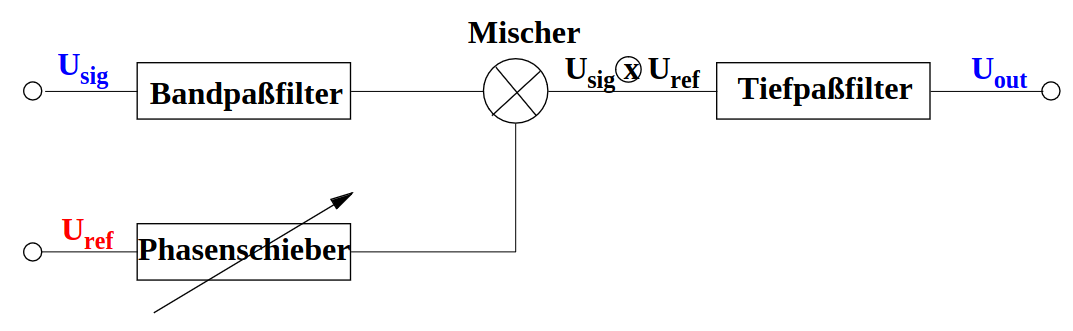
\includegraphics[width=\textwidth]{Versuchsaufbau.png}
    \caption{Aufbau eines Lock-In-Verstärkers}
    \label{fig:Versuchsaufbau}
\end{figure}

\noindent Die Abbildung zeigt, dass das verauschte Nutzsignal $U_\text{Sig}$ zunächst einen Bandpassfilter durchläuft,
welcher sowhol hohe Frequenzen $\left(\omega >> \omega_0\right)$ als auch niedrige Frequenzen $\left(\omega << \omega_0\right)$
\textbf{nicht} passieren lässt. Hierbei bezeichnet $\omega_0$ jene Referenzfrequenz des Referenzsignals $U_\text{Ref}$, mit welcher 
das Netzsignal $U_\text{Sig}$ in dem Mischer multipliziert und somit moduliert wird. Hierbei kann durch den Phasenschieber die Phase  
$\phi$ des Referenzsignals variiert werden, sodass beide Signale $U_\text{Ref}$ und $U_\text{Sig}$ in eine Phase gebracht werden 
$\left(\increment \phi = 0\right)$.Im Anschluss wird der Tiefpassfilter unter der Voraussetzung $\tau = RC >> \sfrac{1}{\omega_0}$ 
$\left(\tau: \text{Zeitkonstante}\right)$ als Integrator des Mischsignals $U_\text{Sig} \times U_\text{Ref}$. Dabei werden 
Rauschbeiträge weitgehend weggemittelt, weshalb ein proportionaler Zusammen zwischen der Eingansspannung und der Ausgangsspannung $U_\text{Out} \propto U_0\cos(\phi)$ existiert.. 
Zusätzlich entscheidet der Tiefpassfilter unmittelbar über die Bandbreite $\increment\nu$ des
Restrauschens. Durch sehr große Zeitkonstanten könne beliebig kleinen Bandbreiten $\increment\nu = \sfrac{1}{\pi\tau}$ erzeugt werden,
wodurch Güten von $Q = 100000$ erreicht werden.\\
Eine beispielhafte Anwendung des Lock-In-Verstärker wird in Abbildung \ref{fig:AWD} aufgezeigt. Hierbei wird das Eingangssignals 
mittels einer sinusförmigen Wechselspannung $U_\text{Sig}(t) = U_{0}\sin(\omega t)$ realisert. Dieses Signal wird nun duch eine
Rechteckspannung $U_\text{Ref}$ der gleichen Frequenz moduliert, welche, wie in der Abbildung zu sehen, bei positiven Signalspannungen
von $U_\text{Sig}(t)$ auf $1$ und bei negativen Signalspannungen auf $-1$ steht.

\begin{figure}
    \centering
    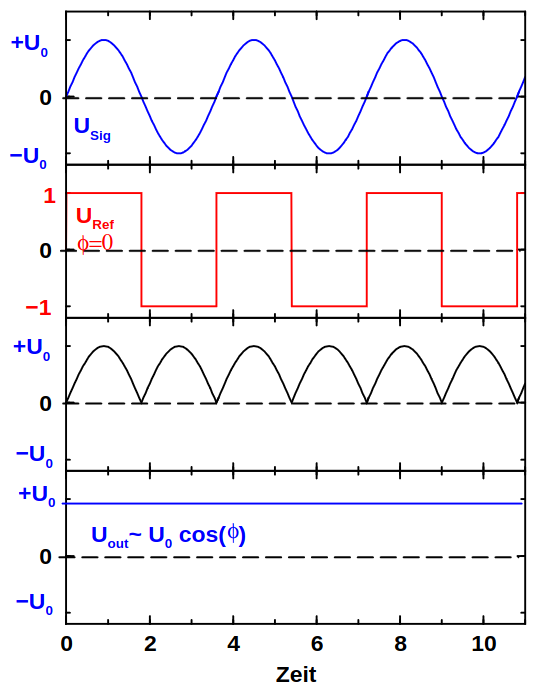
\includegraphics[height=7cm]{AWD.png}
    \caption{Beispielhafte Signalverläufe}
    \label{fig:AWD}
\end{figure}

\noindent Näherungsweise kann der zeitliche Verlauf der Rechteckspannung durch eine Fourrierreihe der ungeraden harmonischen
Grundfrequenzen dargstellt werden:

\begin{equation*}
    U_\text{Ref} = \frac{4}{\pi}\left(\sin(\omega t) + \frac{1}{3}\sin(3\omega t) + \frac{1}{5}\sin(5\omega t) + \dotsc\right)
\end{equation*}

\noindent Das Produkt aus Signal- und Referenzspannung beinhaltet nun die geraden Oberwellen der Grundfrequenz $\omega$ und lässt
sich somit schreiben als

\begin{equation*}
    U_\text{Sig} \times U_\text{Ref} = \frac{2}{\pi}U_0\left(1 - \frac{2}{3}\cos(2\omega t) - \frac{2}{15}\cos(4\omega t) - \frac{2}{35}\cos(6\omega t) + \dotsc\right).
\end{equation*}

Durch eine geeignete Wahl des Tiefpassfilters werden die Oberwellen unterdrückt, sodass die Ausgangsspannung eine zur Eingansspannung
proportionale Spannung darstellt:

\begin{equation*}
    U_\text{Out} = \frac{2}{\pi}U_0\cos(\phi)
\end{equation*}

\noindent Sind beide Signale in Phase $\left(\increment \phi = 0\right)$, so wird die Ausgangsspannung maximal:

\begin{equation*}
    \hat{U}_\text{Out} = \frac{2}{\pi}U_0
\end{equation*}

\section{Vorbereitung}

\section{Fehlerrechnung}
\end{document}